\documentclass[11pt, a4paper, openany]{report}
\usepackage{bookmark}
\usepackage[utf8]{inputenc}
\usepackage[T1]{fontenc}

% LANGUAGE
\usepackage[english]{babel}
\usepackage{enumitem}  % Enumerate improved

% MATH / Others
\usepackage{amsmath, amssymb, amsthm}  % Math symbols
\usepackage{physics}  % \norm and \abs
\usepackage{esvect, cancel}  % Misc., vectors, strikethrough

\newtheorem{thm}{Theorem}
\newtheorem{lem}{Lemma}

\theoremstyle{definition}
\newtheorem{defn}{Definition}
\newtheorem*{prf}{Proof}

\theoremstyle{remark}
\newtheorem{rmk}{Remark}

\usepackage{mhchem}  % Chemistry
\usepackage{siunitx}  % Units SI
\usepackage{minted}  % Code fences ([cache=false])
\setminted[python]{
    fontsize=\footnotesize,
    tabsize=4,
    rulecolor=black,
    xleftmargin=18pt,
    linenos,
    breaklines
}
\usemintedstyle{pastie}

% GEOMETRY
\usepackage[
    paper=a4paper,
    top=2.5cm,
    left=2.25cm,
    headheight=15pt,
    headsep=12pt,
    textwidth=16cm,
    textheight=24cm,
]{geometry}
\usepackage{parskip}  % Reformat paragraphs, no indent first line
\usepackage{enumitem}  % Enumerate improved
\usepackage{scrextend}  % Indent text with addmargin environment
\usepackage{graphicx}  % Include graphics
\graphicspath{{latex-img/}}
\usepackage{caption}  % Caption without figures


% HYPERLINKS
\usepackage{hyperref}
\hypersetup{
    colorlinks=true,
    linktoc=all,
    linkcolor=blue,
}

% HEADERS
\usepackage{fancyhdr}
    \pagestyle{fancy}
    \lhead{Silversmith et al Summary}
    \rhead{Samyak Shah}
    \renewcommand{\footrulewidth}{0.4pt}
    \renewcommand{\headrulewidth}{0.4pt}
\usepackage{etoolbox}  % Define chapter page style
    \patchcmd{\chapter}{\thispagestyle{plain}}{\thispagestyle{fancy}}{}{}

% TITLE PAGE
\title{Silversmith et al Summary}
\author{Samyak Shah}
\date{01/13/2023}

\begin{document}
% TITLE
\maketitle
% TOC
\pagenumbering{gobble}{
    \tableofcontents
    \thispagestyle{plain}
    \cleardoublepage
}
\pagenumbering{arabic}

\section{Abstract}
Two primary limitations of BCIs that have hindered real-world adoption

\begin{enumerate}
    \item Poor long-term reliability
    \item Lengthy daily recalibration times
\end{enumerate}

This paper used a \textbf{128} channel chronic ECoG implant in a \textbf{paralyzed} individual, which allowed for signal stability.
Authors show that long-term closed-loop decoder adaptation, where decoder weights are carried across sessions over multiple days results in a consolidation of neural map and 'plug-and-play' control. Authors also show that in contrast, daily reinitialization led to degradation of performance.

\section{Introduction}
Current intracortical studies must recalibrate the mapping from neural parameters to control dimensions on a daily basis because of recording instability. This generally takes >30min. Past studies (cited in paper) have shown that both setup time and performance stability are strong predictors of real-world use.\\

ECoG is known to be more stable over time, and can enable BCI control. 128 channl ECoG array was implanted in an individual with \textbf{tetraparesis}. They used this to track how the neural representations underlying BCI control changed over time. In particular, they compared decoders \textit{seeded} each day using imagined control with decoders that retained weights. Previous studies have noted \textbf{within-session improvements} using closed-loop decoder adaptation (CLDA), which modifies decoder properties in a stepwise manner as the user learns control. \\

Historically, due to the instability of intracortical spike signals, this required daily CLDA for recalibration. However, it was unclear how to conduct long-term CLDA (ltCLDA), where adaptation occurred over a period of days and weeks. The authors of this study have found that ltCLDA, where weights were carried across days with a long half-life, allowed reliable PnP.\\

The half-life refers to how decoders are updated. Longer half-lives imply greater history of data used to update decoder weights. Additionally, the authors also showed another benefit of consolidation that was \textbf{long term stacking}.
This will allow the ability to add control dimensions over days to existing control.\\

\textbf{It looks like that by consolidation, they are referring to the \textit{consoliation of control strategies}}.

\section{Results}
Experiments were conducted over a period of \( \approx 6 \) months to assess \textbf{two approaches} for decoder adaptation:
\begin{enumerate}
    \item \textbf{Daily Initialization:} Decoder weights were initialized each day by the participant imagining movements (imagining neck and right wrist movements) during passive cursor movements.
    \item \textbf{ltCLDA:} Weights from the previous session were used for the current session. The hypothesis was that it may allow for stablization of decoder weights and improve performance by enforcing a single neural strategy. Basically, by using the weights from the previous session, the user will find a neural strategy that will allow for stable decoder performance across multiple days. 
\end{enumerate}

Experiments were conducted \( \approx 2 \) months after implantation. During these 2 months, patients had a recovery period followed by \textbf{general exposure} to cursor control. \\

The first experiments were performed using daily initialization. The Fitt's information transfer rate (ITR) remained constant over this time. During ltCLDA, it was noted that there was now a 'convergence' of decoder weights. Basically, the angles between the decoder weight subspaces converged to 0.\\

\textbf{[Note to self]: Make sure you understand how exactly they are determining the angle between the decoder weight subspaces}\\

To quantify decoder convergence, the authors examined 'within-day decoder differences'. This refers to the angle of the decoder at the beginning of each day in Figure 1, \textbf{plot e}. This measure was compared during the first 5 days vs the last 5 experimental days. There was a significant decrease in within-day decoder differences.\\

Additionally, There was a significant improvement in Fitts' ITR during the last 5 days compared to the performance during daily initialization.\\

The authors state that there was no evidence that the participant was using overt movement strategies. 

\begin{defn}[Fitt's ITR]
    Fitt's ITR was originall proposed in 1954 by Paul Morris Fitts as a metric to quantify the difficulty of a \textbf{target selection task}. The metric is based on an analogy to information theory, where
    the distance to the center of the target \( (D) \) is like a signal and the tolerance of the target \( (W) \) is like noise.
    The metric is Fitts' index of difficulty (\( ID \) in bits):
    \[ \mathrm{ID} = \log_2 \left( \frac{2D}{W} \right) \]
    Fitts also proposed an \textit{index of performance} (\( IP \) in bits per second) as a measure of human performance. The metric combines a task's index of difficulty \( (ID) \) with the movement time (\( (MT) \) in seconds) in selecting the target. Thus,
    \[ IP = \left( \frac{ID}{MT} \right) \]
    As of today, \( IP \) is more commonly known as \textit{throughput} \( (TP) \).
    The equation that expresses the relationship between \( MT \) and the \( D \) and \( W \) task parameters is
    \[ MT = a + b \cdot ID = a + b \cdot \log_2 \left( \frac{2D}{W} \right) \] where
    \begin{itemize}
        \item \( MT \) is the average time to complete the movement in seconds.
        \item \( a \) and \( b \) are constants that depend on the choice of input device and are usually determined empirically by regression analysis. \( a \) usually is interpreted as the \textbf{delay} while \( b \) is usually described as the \textbf{acceleration}.
        \item \( ID \) is the index of difficulty.
        \item \( D \) is the distance from the starting point to the center of the target.
        \item \( W \) is the width of the target \textbf{measured along the axis of motion}. \( W \) can also be thoought of as the allowed error tolerance in the final position, since the final position of motion must fall within \( \pm \frac{W}{2} \) of the target's center.
    \end{itemize}
\end{defn}

\begin{rmk}
    The formulation of Fitts' index of difficulty used for BCI research is called the \textbf{Shannon formulation}:
    \[ ID = \log_2 \left( \frac{D}{W} + 1 \right) + 1\]
    this is so named for it's resemblance to the Shannon-Hartley theorem, which describes the transmission of information using bandwidth, signal strength and noise. In Fitts' law, the distance represents signal strength, while target width is noise. Note that \textbf{no formal mathematical connection was established between Fitts' law and the Shannon-Hartley theorem}.
\end{rmk}

\hyperref[https://www.yorku.ca/mack/JMB89.html]{Explanation of the relation between Fitt's Law and Information Theory}

\begin{rmk}[Adjustment for Accuracy]
    We can adjust Fitts' law for accuracy by varying the specified or set target width (akin to noise) according the the spatial variability in the patient's output responses over a sequence of trials. 
    The output, or \textbf{effective target width} \( W_e \) is derived from the distribution of "hits". The movement amplitudes are analogous to "signals" and the endpoint variability is analogous to "noise". \\

    The information theorem underlying Fitts' Law assumes that the signal is "perturbed by white thermal noise". The analogous requiremente in motor tasks is a Gaussian or normal distribution of hits - a property observed by numerous researchers. \\

    The entropy, or information, in a normal distribution is \( \log_2 \left( \sqrt{2 \pi e} \sigma \right) = \log_{2} \left( 4.133 \sigma\right) \), where \( \sigma \) is the standard deviation in the nit of measurement. Splitting the constant 4.133 into a pair of z-scores for the unit-normal curve \( \sigma = 1 \), one finds that \( 96\% \) of the total area is bounded by \( -2.066 < z < +2.066 \). In other words, a condition that target width is analogous to noise is that the distribution is normal with with \( 96\% \) of hits fall within the target area.\\

    There are two ways for determining the effective traget width
    \begin{enumerate}
        \item \textbf{The standard deviation method}: In this method, if the standard deviation of one of the end-point coordinates is known, \( W_e = 4.133 \cdot \sigma \). 
        \item \textbf{The discrete-error method}: If only the percentage of errors is known, the method uses a table of z-scores for areas under the unit-normal curve. I \( n \) percent errors are observed over a sequence of trials for a particular \( A-W \) condition, determine \( z \) such that \( \pm z \) contains \( 100-n \) percent of the area under the normal curve. Then, \( W_e = W \cdot \frac{2.066}{z} \).
    \end{enumerate}

    As an example, if \( 2\% \) errors occur on a sequence of trials when selecting a \( 5 \)cm wide target, then 
    \[ W_e = \frac{2.066}{z} \cdot W = \frac{2.066}{2.326} \cdot 5 = 4.45 \mathrm{cm} \]

    A more detailed explanation of Fitts' Law may be found \hyperref[https://onlinelibrary.wiley.com/doi/book/10.1002/9781118976005]{here}.

\end{rmk}

The authors also quantified decoder adaptation by \textbf{computing the change in angle} between the decoder subspaces each day (90 degrees indicates orthogonality and 0 degrees indicates no change). Notably, the weights appeared to reset towards orthogonality at the start of each daily session. 

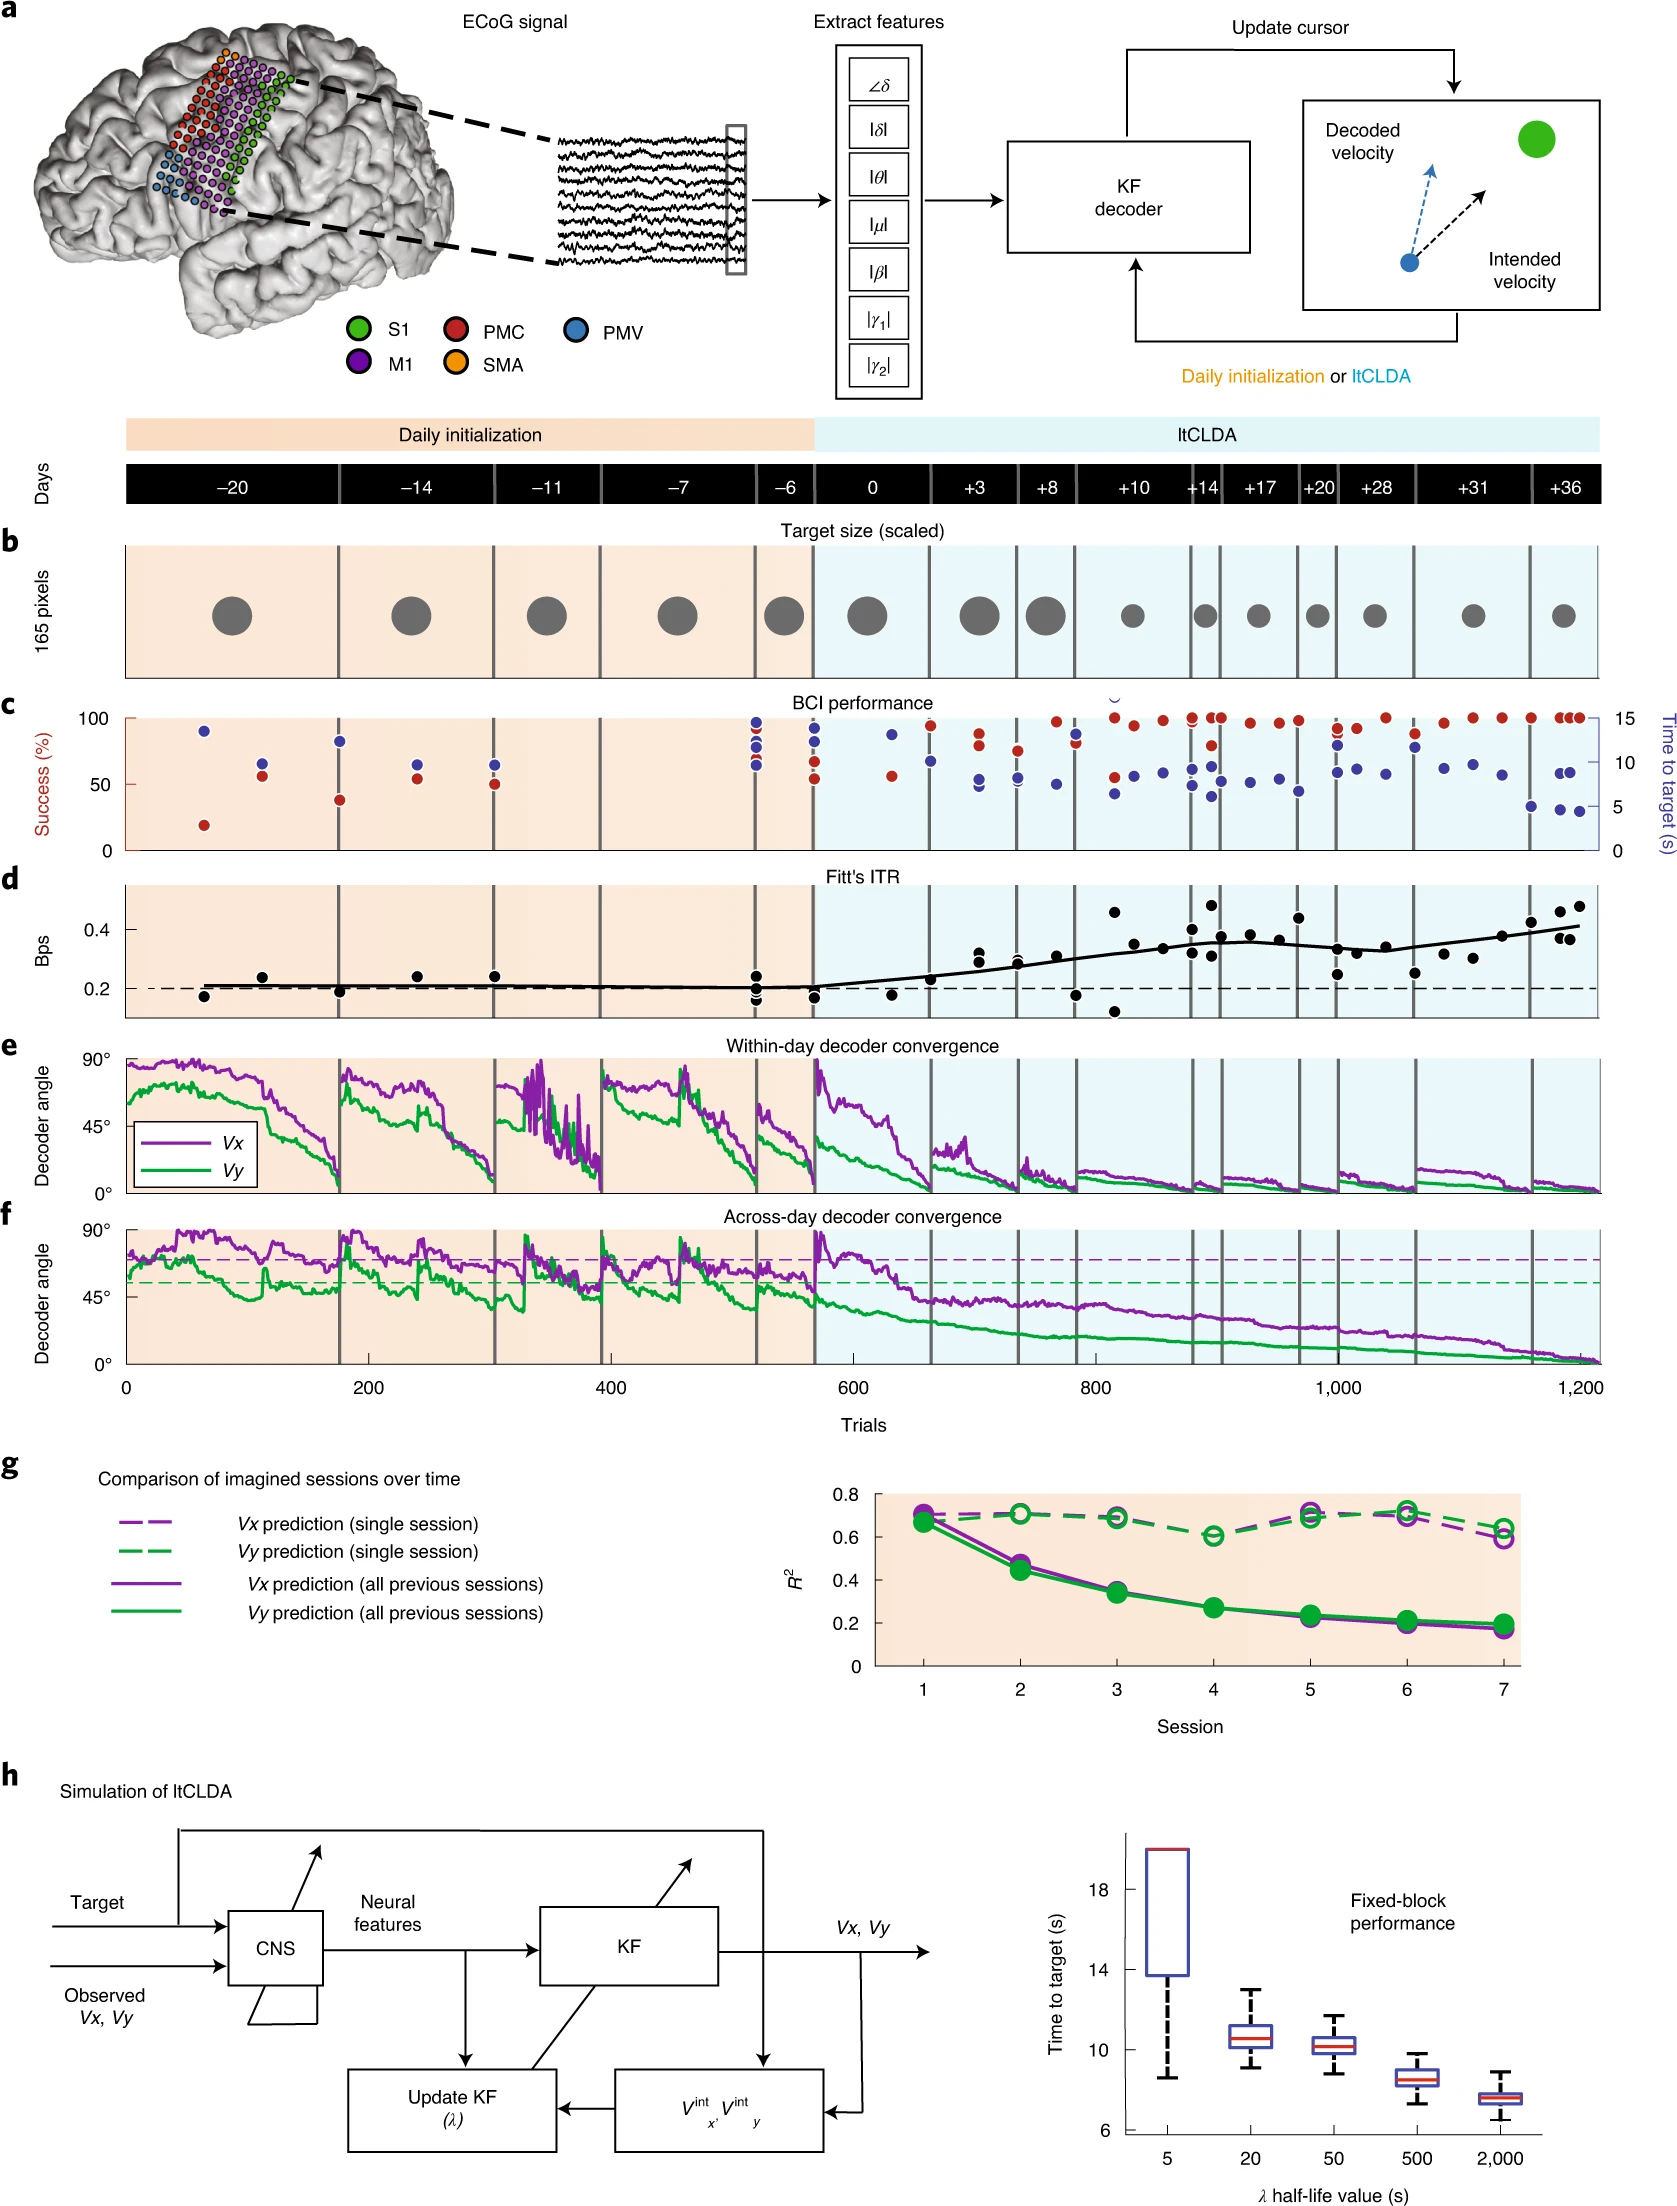
\includegraphics[width=\linewidth]{images/silversmith1.png}

The figure above summarizes the results of the experiments. \textbf{Plot b} shows the relative sizes of the center out task. Note that this will affect the Fitts' ITR. \textbf{Plot c} shows the performance of the BCI measured during 'fixed' control, where the decoder parameters were held constant. There are some days without values, i.e. -11 and -7. These are days wherein the patient had such poor control, that they could not even complete a block. 
\textbf{Plot d} shows the BCI performance over time as measured by changes in Fitts' ITR. \textbf{Plot e} shows the changes in angle between \( x \)-velocity \( (Vx) \) and \( y \)-velocity \( Vy \) decoder weights over time. The angle between the decoder at each trial and the final decoder is marked by the vertical line. \textbf{I'm not sure what the decoder weights are being compared to.} It seems as though the comparisons are being performed between
the the weights of each trial and the final trial of the day. \textbf{Plot f} denotes the angle between the decoder at each trial and the final decoder at the end of ltCLDA, that is, day 36. \textbf{Plot g} denotes the \( R^{2} \) values, computed by fitting a decoder to each respective \textbf{imagined} movement session (dashed lines) or by fitting a decoder to using all previous imagined movement sessions (solid lines). 

\subsection{How \( R^{2} \) is estimated for imagined cursor movements }
The \( R^{2} \) values in Figure 1 plot g was generated using 'leave-out' multivariate regression between all features and the displayed \( Vx \) and \( Vy \) cursor velocities. 
For single sessions, the authors used 80\% of the data to build a multivariate regression model to predict \( Vx \) and \( Vy \) separately. \textbf{I am guessing that this is the feature data, i.e. High Gamma activity, etc.} \( R^{2} \) values represent the match between the predicted and the actual values for the \textbf{left-out data}. This was repeated 5 times per session. The multiple-session curve (solid line), sessions were added in. The leave-out validation was \textbf{randomly interspersed} in the respective combined datasets.

Note that when data was pooled from multiple days in a systematic manner, the \( R^{2} \) value was progressively lower with the addition of each day. The authors interpreted this to mean that the relationship between neural features and the cursor velocity during imagined sessions was not stable across days; thus, a regression model that pooled days performed worse than a single session.

\subsection{Decoder convergence comparison}
To compare decoder convergence, during daily initialization and ltCLDA, the convergence tragjectories (decoder angles relative to the final trial) during the first 5 days of both daily initialization and ltCLDA. There was a significant difference in the convergence trajectories between the two for both \( Vx \) and \( Vy \). \\

When a linear model was used to quantify the rate of convergence, the authors found significantly faster convergence rates during ltCLDA when compared to daily initialization. The decoder angles are presented in plot 1e.\\

\textbf{Together, these results indicate that there was a sustained convergence of weights to a stable decoder with ltCLDA}.\\

The authors suggest that long time constants for decoder updates (such as 500-5,000s) are important. \( \lambda \), the half life, determines how the past data is exponentially weighted. Intuitively, the half life is a paramete (in units of time), that reduces the contribution of previously estimated decoders by a factor of two at the current time step. In computational experiments, the authors found that ltCLDA with higher \( \lambda \) values in the setting of a converging neural strategy translated to better fixed control.\\

The hypothesis is hat ltCLDA provides a smoothly moving goal for the simulated user during training, allowing a better estimate of decoder weights to match overall user strategy. With a smaller \( \lambda \), the target is highly variable, and thus likely to result in impoverished learning. \\

Finally, the authors also tracked ltCLDA and its corresponding BCI performance over multiple months. The results showed relatively little variation in decoder weights and kalman gain over time with continued ltCLDA, and fixed performance continued to be stable. 


\section{Methods}
\subsection*{Center-out task}
A target was placed at the center of the screen, and \textbf{eight} outer targets were placed on a circle at 45 degree intervals. \textbf{Targets were presented in blocks of eight trials}. In a single trial, each outer target was presented once in a random order. To complete a trial, the center of the cursor had to \textbf{overlap with the target} (read, not overlap with the center of the target) for a single 200-ms time bin. \\

A \textbf{trial} consisted of one reach to the center target and another reach to the instructed outer target. This is interesting, because normaly trials will be switched, i.e. reach to the outer target first. If the participant failed to select the targeet within the itime limit, the trial was registered as an error, and the cursor was reset to center. My guess is that the first reach was not counted as a trial. \\

\textbf{Note, that there was no overt movement in any of the trials. All trials were imagined}

There were three types of blocks
\begin{enumerate}
    \item \textbf{Imagined Control Blocks:} In these blocks, the participant imagined moving their arm up and down to move the cursor up and down, and moving their head left and right to move the cursor left and right. \textbf{The participant did not move during this task}. The participant was anslo unable to move at speeds comparable to the virtual cursor movements. I wonder if this helped decoding performance as the movements were more 'aggressive'. 
    \item \textbf{CLDA Control Blocks:} For CLDA control blocks, the decoder parameters were updated during each time bin (we expand on this in the cursor control algorithm). For some of the days, (-20 through -6 for daily initialization and 0 through +2 for ltCLDA), each session began with a small level of assistance (~5-10 percent), decayed within a few blocks. 
    \item \textbf{Fixed Control Blocks:} During fixed control blocks, the participant was in full control of the cursor. Decoder parameters fixed. 
\end{enumerate}

\subsection{Point-and-click task}
Gray squares were laid out in a 4x4 grid. Target square would turn green. Initially, patients were just asked to hold the cursor within the target, with successful selection occurring if held for a duration of 600-1000ms. Later, participant was asked to make a click, and the cursor position was reset to center. The imagined movement for the neural click was clicking a mouse. 

\section{Kalman Filter as a BCI Decoder}
In this paper, the relationship between the neural fetaures \( y \) and the cursor kinematics \( x \) was modeled using the equation
\[ y_t = C x_t + q_t \]
\begin{itemize}
    \item \( q \in  N(0, Q) \) is the measurement noise
    \item \( y \in  R^{p \times 1} \) is a \( p \) dimensional vector of \( p \) neural features
    \item \( x = [x_{pos}, y_[pos], x_{vel}, y_{vel} 1]^{\top} \) is the state vector describing the 2D kinematics of the cursor, with the last entry in \( x \) accounting for the mean neural feature value
    \item \( C \in R_{p \times 5} \) is the observation matrix relating the neural features to the cursor state. 
\end{itemize}

A velocity-Kalman Filter was utilized where it was assumed that neural features are related to the \( x \) and \( y \) velocities of the cursor. This means the first two columns of \( C \) will be vectors of zero. For any neural feature \( i \) and at any time \( t \)
\[ y_i(t) = C_{x_{vel}(i)} x_{vel}(t) + C_{y_{vel}(i)}y_{vel}(t) + C_{0(i)} + q(t) \]
Note that \( C_{0(i)} \) is the mean of feature \( y_i \)\\

Additionally, the cursor kinematics/cursor state was assumed to evolve dynamically through time,
\[ x_t = A_{x_{t-1}} + w_t \]
where 
\begin{itemize}
    \item \( w \in  N(0, W) \) is the state noise. 
    \item \( A \in  R^{5 \times 5} \) is the state evolution matrix that models cursor kinematics to follow simple laws of motion:
    \[ M = \begin{pmatrix}
    1 & 0 & dt & 0 & 0\\
    0 & 1 & 0 & dt & 0\\
    0 & 0 & a & 0 & 0\\
    0 & 0 & 0 & a & 0\\
    0 & 0 & 0 & 0 & 1
    \end{pmatrix} \] 
    Note that the \( a \)'s are not necessarily the same as acceleration, but rather they may be thought of as a damping constant.
\end{itemize}

the cursor velocity is hidden, but estimated from the measured neural data. Cursor position was then estimated by integrating the velocity. At the start of the trial, the cursor position was set to the center of the screen (0, 0), and then the new position was computed using integration
\[ \hat{x}_{pos}(t) = \hat{x}_{pos}(t-1) + \hat{x}_{vel}(t) \cdot dt \]
\[ \hat{y}_{pos}(t) = \hat{y}_{pos}(t-1) + \hat{y}_{vel}(t) \cdot dt \]

Note that \( dt \) is the sampling rate of the decoder. As a velocity Kalman Filter was used, it was assumed that there was only uncertainty in the velocities of the cursor state. As a result, the \( W \) matrix was fixed to be

\[ W = \begin{pmatrix}
0 & 0 & 0 & 0 & 0\\
0 & 0 & 0 & 0 & 0\\
0 & 0 & w & 0 & 0\\
0 & 0 & 0 & w & 0\\
0 & 0 & 0 & 0 & 0
\end{pmatrix} \]



\end{document}